\begin{figure*}[b]
	\centering
	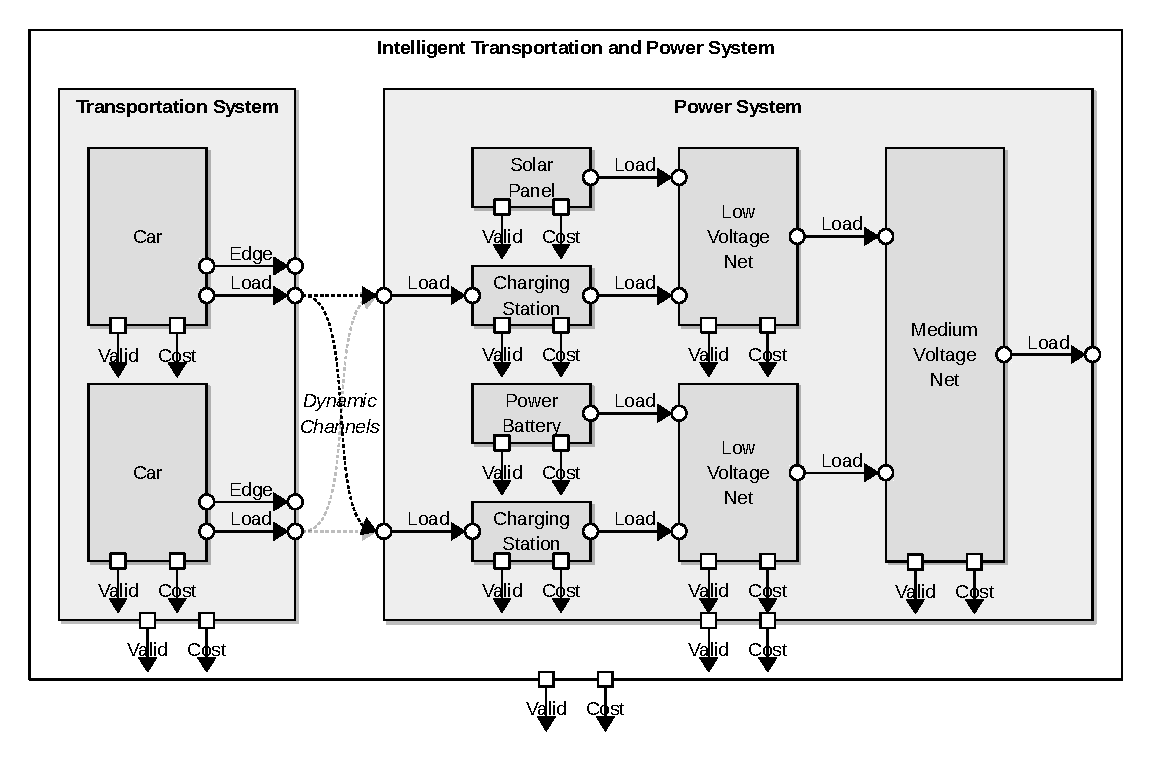
\includegraphics[width=\textwidth]{../gfx/model.pdf}
	\caption{Overview of the holistic modeling approach including transportation and power system connected by dynamic channels.}
	\label{fig:model}
\end{figure*}

\section{Transportation and power systems modeling}
\label{section:contribution}

Based on the underlying systems modeling technique (see Sec.~\ref{section:foundation}), we propose an integrated transportation and power system model as shown in Figure~\ref{fig:model}. At its root, the model defines an intelligent transportation and power system component, which contains separate components for the transportation and the power system. The transportation system component comprises the individual car components traveling along the traffic infrastructure. Similarly, the power system component includes the individual electric components, such as static loads, solar panels, power batteries and charging stations. Furthermore, the power system component contains the electric infrastructure consisting of low-voltage and medium-voltage net components. Parametrization allows one to instantiate all components using reference configurations, i.e. predefined parameter valuations. Subsequently we describe the different components of the model in terms of their parameters, ports, channels and behavior. Furthermore, for each parameter we provide a description as well as reference configurations.

\subsubsection*{Intelligent transportation and power system}
\label{section:intelligent_system}

The intelligent transportation and power system $IS$ component contains the transportation system $TS$ and the power system $PS$ (see following table). Furthermore, the $IS$ defines dynamic channels between the car load outputs of $TS$ and the charging station load inputs of $PS$. Consequently, each car is connected to each charging station statically, but loads are forwarded only to the connected charging station dynamically. Therefore, the dynamic channel conditions test whether the car position (i.e.\ the edge output, see Sec.~\ref{section:car}) matches the charging station position (i.e.\ some constant edge, see Sec.~\ref{section:charging_station}). Furthermore, the intelligent transportation and power system $IS$ specifies a cost output which aggregates the cost of the transportation system $TS$ and the power system $PS$ using the weights $w\_TS$ and $w\_PS$. On this cost output a minimization objective is defined through annotation. Finally, no additional constraints are defined on system state and behavior.

\subsubsection*{Transportation system}

The transportation system component $TS$ comprises the traffic infrastructure $TN$ as well as the car components $C$ (see following table). The traffic infrastructure $TN$ is modeled as directed graph $G = (V,E)$ with nodes $V$ and edges $E \subseteq V \times V$. Here, nodes $v,w \in V$ represent reference points in the traffic infrastructure such as intersections. Moreover, nodes define an absolute position in real-world coordinates (i.e. latitude, longitude, and elevation). In contrast, edges $(v,w) \in E$ represent road segments between source nodes $v$ and target nodes $w$. Furthermore, edges define their number of lanes as well as their road type (e.g.\ residential streets or stations). The cars $C$, on the other hand, can be configured by means of the parameters $Car\_Number$ and $Car\_Frequency$. While the former defines the total number of cars, the latter models a distribution over available car reference configurations. Finally, the transportation system $TS$ defines a cost output which aggregates the cost of the individual cars $C$. To ensure valid behavior, $TS$ additionally implements a constraint over the car positions which calculates the largest number of pair-wise overlapping cars per segment $(v,w) \in E$ and compares it to the available number of lanes.

\subsubsection*{Car}
\label{section:car}

Cars $C$ represent atomic components in our system model and are defined in terms of a range of parameters shown in the following table. Key physical parameters are their $Length$ and $Weight$. Moreover, they contain a battery with predefined state of charge $SOC$. For battery charging and discharging they specify the parameter $Charge\_Rate$. During simulation, when the time point $Departure\_Time$ is passed the car starts traveling from origin $Origin$ to destination $Destination$. Origins, destinations and current position of cars are edges $v \in V$ of the traffic infrastructure $TN$. When starting to travel, the car position equals the origin, while subsequent positions are selected from a set of possible routes. The set of possible routes equals to the $k \in \mathbb{N}$ shortest paths from the current position to the destination or the nearest charging station. Of these alternatives one route is selected randomly depending on the parameter $CS\_Selection$. If the state of charge falls below a specified percentage described by the parameter $Range\_Anxiety$, the route selection probability shifts towards preferring the nearest charging station. While driving along the traffic infrastructure, cars consume energy. The energy consumption is based on the energy efficiency parameter $Efficiency$, the traveled elevation profile, car weight as well as the randomly selected speed. Hereby, the speed is limited by the parameter $Speed\_Max$. Both energy consumption and possibly production are applied to the state of charge. Consumption occurs during driving or during discharge at charging stations. Production occurs during driving (i.e.\ energy recuperation) or during charging at charging stations instead. To ensure valid behavior, a constraint tests whether the state of charge lies within a constant minimum $SOC\_Min$ and maximum $SOC\_Max$. When connected to a charging station, the (dis-)charging decision is taken randomly with uniform distribution. If the car charges, a predefined load (i.e.\ charge rate) is transferred from the charging station to the car. If the car discharges, a predefined load is transferred from the car to the charging station instead. Furthermore, the car can choose an idle state, in which case no load is transferred between car and charging station. Finally, the car objective includes multiple cost factors. Generally, car cost only accumulate after its departure time $Departure\_Time$ has passed. The first cost factor evaluates the car's state of charge with respect to the car's maximum state of charge. The second cost factor aggregates the time needed to reach the destination $Destination$. And the third cost factor measures the energy consumption in relation to the maximum energy consumption. The cost factors are aggregated and weighted using the parameters $w\_SOC$, $w\_Time$ and $w\_Power$.

\subsubsection*{Power system}

The power system component $PS$ represents the overall electric infrastructure including individual electric devices as well as low-voltage nets $LV$ and medium-voltage nets $MV$ (higher voltage nets are omitted currently). Currently supported devices include static loads $SL$, solar panels $SP$, power batteries $PB$ and charging stations $CS$. Furthermore, the power system can be configured using a number of parameters which are summarized in the following table. At its interface the power system specifies a cost output that aggregates the cost of the power batteries $PB$, solar panels $SP$, charging stations $CS$ as well as low- and medium-voltage networks $LV$/$MV$. In principle, different aggregation schemes can be used. Furthermore, it forwards the load of the medium-voltage network representing the final load balance.

\subsubsection*{Low/medium-voltage nets}

In our model, low- and medium-voltage nets $LV$/$MV$ are modeled in terms of atomic components receiving loads from all connected electric devices and providing an aggregate load output to the upper voltage level. Note that connected electric devices can be lower voltage net components as well. The following table summarized the parameters used for configuring net components. During simulation, low-voltage nets sum up the loads of all connected static loads, power batteries, solar panels, and charging stations to yield the load output. The medium-voltage net aggregates the loads of all low-voltage nets instead. Based on the aggregated load, a net's cost output is specified relative to the total net capacity $Capacity$ (i.e.\ the closer to the capacity, the worse). Then, each net's cost output is dampened by the weight parameter $w\_Balance$. Finally, to ensure valid behavior a constraint tests if a net's aggregated load as well as all connected loads lie within the net's total capacity $Capacity$. More information on the model can be found in~\cite{hackenberg2012applying}.

\subsubsection*{Static load}

Static loads $SL$ (see following table) aggregate a wide range of electric devices, which cause non-controllable loads (such as conventional light bulbs, washing machines or dish washers). Consequently, they abstract from specific details about different electric devices, i.e. producers and consumers, reducing the available information to their load per time instant only. The result of this aggregation can be defined in terms of a load profile $L = (l_t)_{0 \leq t \leq n}$ with $t,n \in \mathbb{N}$ representing current and maximum time points and $l_t \in \mathbb{R}$ representing positive or negative loads with unit kW/h. Based on the parameters $Power\_Scale$ and $Profile$ static load components generate a predefined load profile. Both parameters allow one to vary static (i.e.\ non-controllable) load in different scenarios easily. In particular, the scale factor serves to dampen the static profile.

\subsubsection*{Power battery}

Power battery components $PB$ represent stationary devices acting as both producers and consumers within the electric infrastructure (e.g.\ lead-acid batteries). The following table shows the parameters that can be used to configure batteries.In each simulation step, power batteries choose randomly between charging, discharging or idle mode. In terms of their probability these modes are distributed uniformly. Depending on the selected mode, energy consumption (i.e.\ negative load) or production (i.e.\ positive load) can be observed on the low-voltage net side. Furthermore, production and consumption takes effect on the internal state of charge, which is initialized with the $SOC$ parameter. The speed of charging and discharging is configured by means of the $Charge\_Rate$ parameter. Consequently, our model assumes constant charge and discharge speed. While charging, only a limited amount of energy is transferred to the state of charge. This amount can be configured using the $Battery\_Efficiency$ parameter. Finally, the state of charge is subject to loss over time configured with the $Battery\_Loss$ parameter. To ensure valid behavior, a constraint tests whether the state of charge lies within a constant minimum and maximum expressed through the parameters $SOC\_Min$ and $SOC\_Max$. Detailed information about the battery model can be found in~\cite{hackenberg2014rapid}.

\subsubsection*{Solar panel}

Solar panel components $SP$ are electric devices, which represent one class of renewable energy producers with a defined yield within the electric network. They are characterized by the three parameters listed in the following table. Based on their specific power scale $Power\_Scale$, solar panels produce a positive load peaking at the mean time point $Mean$ with a variance $Variance$. Moreover, based on probabilistic selection solar panels can choose to dampen their production (known as maximum power point tracking). The probability of the choices is uniformly distributed. Detailed information about the model can be found in~\cite{hackenberg2014rapid}.

\subsubsection*{Charging station}
\label{section:charging_station}

Finally, charging station components $CS$ represent electric devices acting as consumers or producers within the electric network, while facilitating the charging process of the cars $C$ of the transportation system $TS$. They are assigned a physical location, i.e.\ an edge $(v,v) \in E$ of the traffic infrastructure $TN$ with zero length (i.e.\ same source and target node $v \in V$). In terms of behavior, charging stations $CS$ can exhibit zero, negative or positive load to the low-voltage net. Based on dynamic connection to cars (see Sec.~\ref{section:intelligent_system}), a charging station's behavior is determined by the selected charging mode of the car $C$. Charging stations may act as consumers, when energy is transferred from the charging station to the car. In contrast, the stations also may act as producers, when energy is transferred from the car to the charging station. The respective energy transfer rate is specified by means of the $Charge\_Rate$ parameter.